% syntralinepp_architecture.tex
% Detailed, non-overlapping, one-diagram-per-page architecture document
% NOTE: This file is designed to compile cleanly with generous spacing.
%       Each diagram sits on its own page via \newpage.

\documentclass[11pt]{article}
\usepackage[a2paper,margin=18mm]{geometry}
\usepackage[T1]{fontenc}
\usepackage{lmodern}
\usepackage{microtype}

\usepackage{tikz}
\usetikzlibrary{arrows.meta,positioning,fit,calc,shapes.multipart}

\pagestyle{empty}

% ---------- Global spacing helpers ----------
\setlength{\parindent}{0pt}
\setlength{\parskip}{6pt}

% ---------- Styles ----------
\tikzset{
  font=\small,
  box/.style={
    draw,
    rounded corners=3pt,
    align=center,
    minimum width=48mm,
    minimum height=12mm,
    inner sep=6pt
  },
  wide/.style={
    draw,
    rounded corners=3pt,
    align=left,
    minimum width=140mm,
    inner sep=8pt
  },
  small/.style={
    draw,
    rounded corners=3pt,
    align=center,
    minimum width=34mm,
    minimum height=10mm,
    inner sep=4pt,
    font=\scriptsize
  },
  note/.style={
    draw,
    rounded corners=3pt,
    align=left,
    minimum width=60mm,
    inner sep=6pt,
    font=\scriptsize
  },
  group/.style={
    draw,
    rounded corners=4pt,
    inner sep=6pt
  },
  arrow/.style={-Latex, thick},
  dashedarrow/.style={-Latex, thick, dashed}
}

\begin{document}

% =============================================================================
% Diagram 1 — End-to-End Compiler Overview (DETAILED)
% =============================================================================
\section*{Diagram 1 — SyntraLine++ End-to-End Compiler Pipeline (Detailed)}

\begin{center}
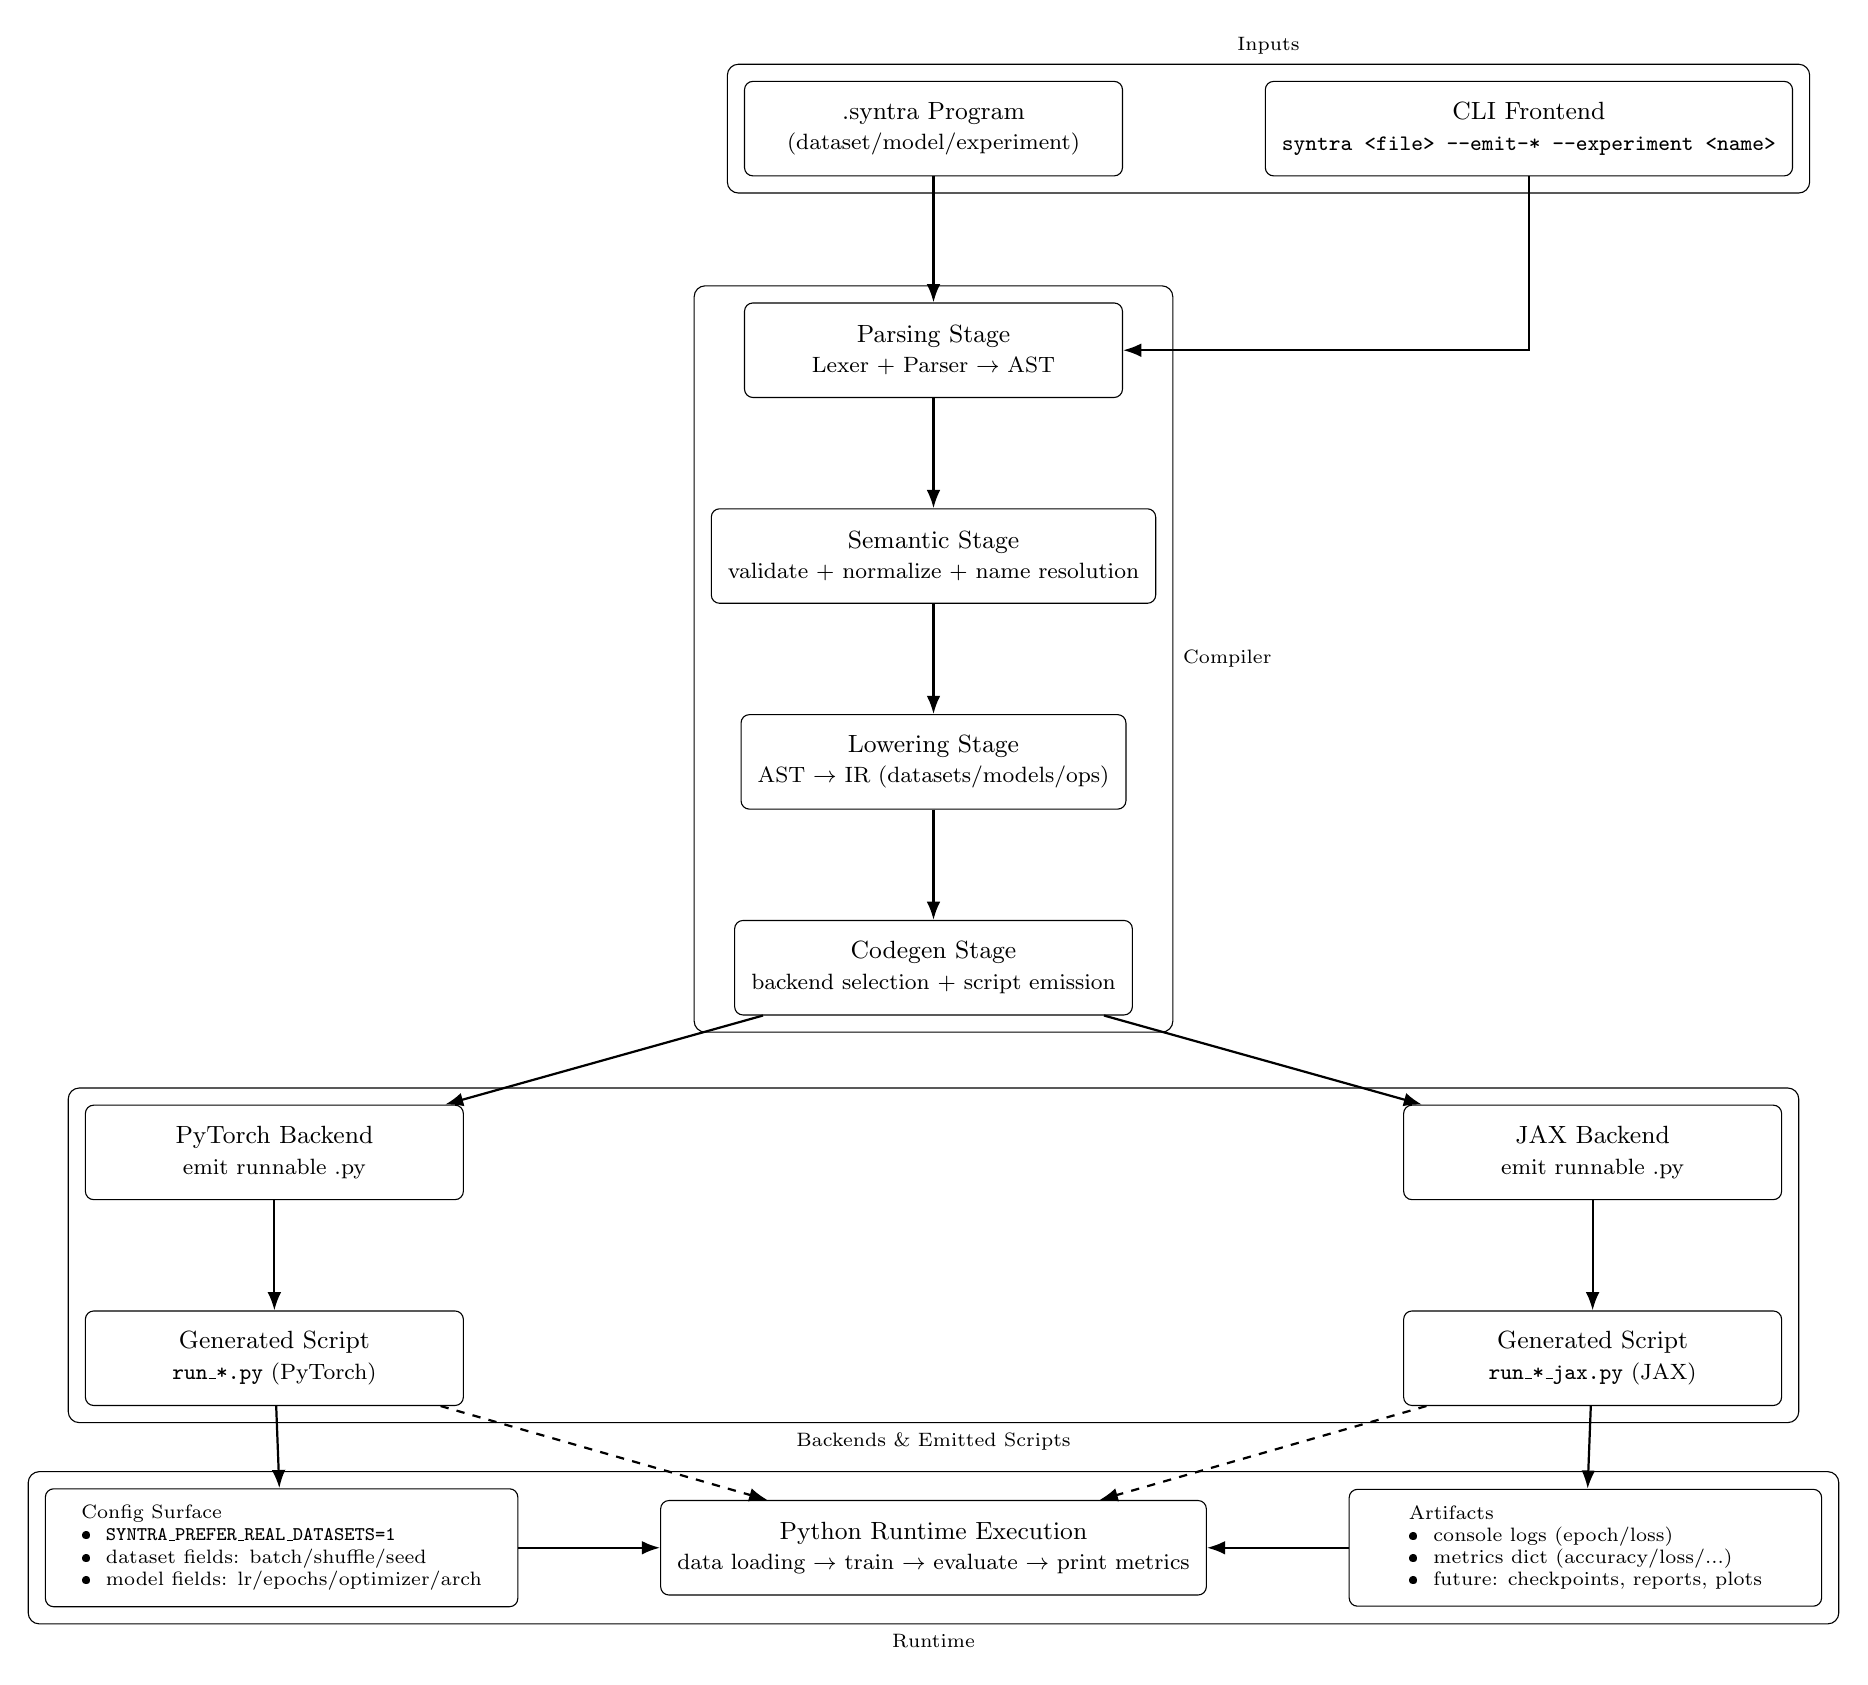
\begin{tikzpicture}[node distance=14mm]

% --- Top row: inputs + CLI
\node[box] (src) {.syntra Program\\\footnotesize (dataset/model/experiment)};
\node[box, right=18mm of src] (cli) {CLI Frontend\\\footnotesize \texttt{syntra <file> --emit-* --experiment <name>}};

% --- Middle: compiler pipeline
\node[box, below=16mm of src] (parse) {Parsing Stage\\\footnotesize Lexer + Parser $\rightarrow$ AST};
\node[box, below=of parse] (sem) {Semantic Stage\\\footnotesize validate + normalize + name resolution};
\node[box, below=of sem] (lower) {Lowering Stage\\\footnotesize AST $\rightarrow$ IR (datasets/models/ops)};
\node[box, below=of lower] (codegen) {Codegen Stage\\\footnotesize backend selection + script emission};

% --- Backends and outputs
\node[box, below left=16mm of codegen, xshift=-23mm] (pt) {PyTorch Backend\\\footnotesize emit runnable .py};
\node[box, below right=16mm of codegen, xshift=23mm] (jax) {JAX Backend\\\footnotesize emit runnable .py};

\node[box, below=14mm of pt] (ptout) {Generated Script\\\footnotesize \texttt{run\_*.py} (PyTorch)};
\node[box, below=14mm of jax] (jaxout) {Generated Script\\\footnotesize \texttt{run\_*\_jax.py} (JAX)};

% --- Runtime + artifacts
\node[box, below=18mm of $(ptout)!0.5!(jaxout)$] (runtime) {Python Runtime Execution\\\footnotesize data loading $\rightarrow$ train $\rightarrow$ evaluate $\rightarrow$ print metrics};
\node[note, right=18mm of runtime] (artifacts) {Artifacts\\
\textbullet\; console logs (epoch/loss)\\
\textbullet\; metrics dict (accuracy/loss/...)\\
\textbullet\; future: checkpoints, reports, plots};

% --- Control signals / config
\node[note, left=18mm of runtime] (config) {Config Surface\\
\textbullet\; \texttt{SYNTRA\_PREFER\_REAL\_DATASETS=1}\\
\textbullet\; dataset fields: batch/shuffle/seed\\
\textbullet\; model fields: lr/epochs/optimizer/arch};

% --- Arrows
\draw[arrow] (src) -- (parse);
\draw[arrow] (cli) |- (parse);
\draw[arrow] (parse) -- (sem);
\draw[arrow] (sem) -- (lower);
\draw[arrow] (lower) -- (codegen);
\draw[arrow] (codegen) -- (pt);
\draw[arrow] (codegen) -- (jax);
\draw[arrow] (pt) -- (ptout);
\draw[arrow] (jax) -- (jaxout);
\draw[arrow] (ptout) -- (config);
\draw[arrow] (config) -- (runtime);
\draw[arrow] (jaxout) -- (artifacts);
\draw[arrow] (artifacts) -- (runtime);
\draw[dashedarrow] (ptout) -- (runtime);
\draw[dashedarrow] (jaxout) -- (runtime);

% --- Grouping boxes (fit)
\node[group, fit=(src)(cli), label={[font=\scriptsize]above:Inputs}] {};
\node[group, fit=(parse)(sem)(lower)(codegen), label={[font=\scriptsize]right:Compiler}] {};
\node[group, fit=(pt)(jax)(ptout)(jaxout), label={[font=\scriptsize]below:Backends \& Emitted Scripts}] {};
\node[group, fit=(runtime)(config)(artifacts), label={[font=\scriptsize]below:Runtime}] {};

\end{tikzpicture}
\end{center}

\newpage

% =============================================================================
% Diagram 2 — Parsing and AST Construction (DETAILED)
% =============================================================================
\section*{Diagram 2 — Parsing and AST Construction (Detailed)}

\begin{center}
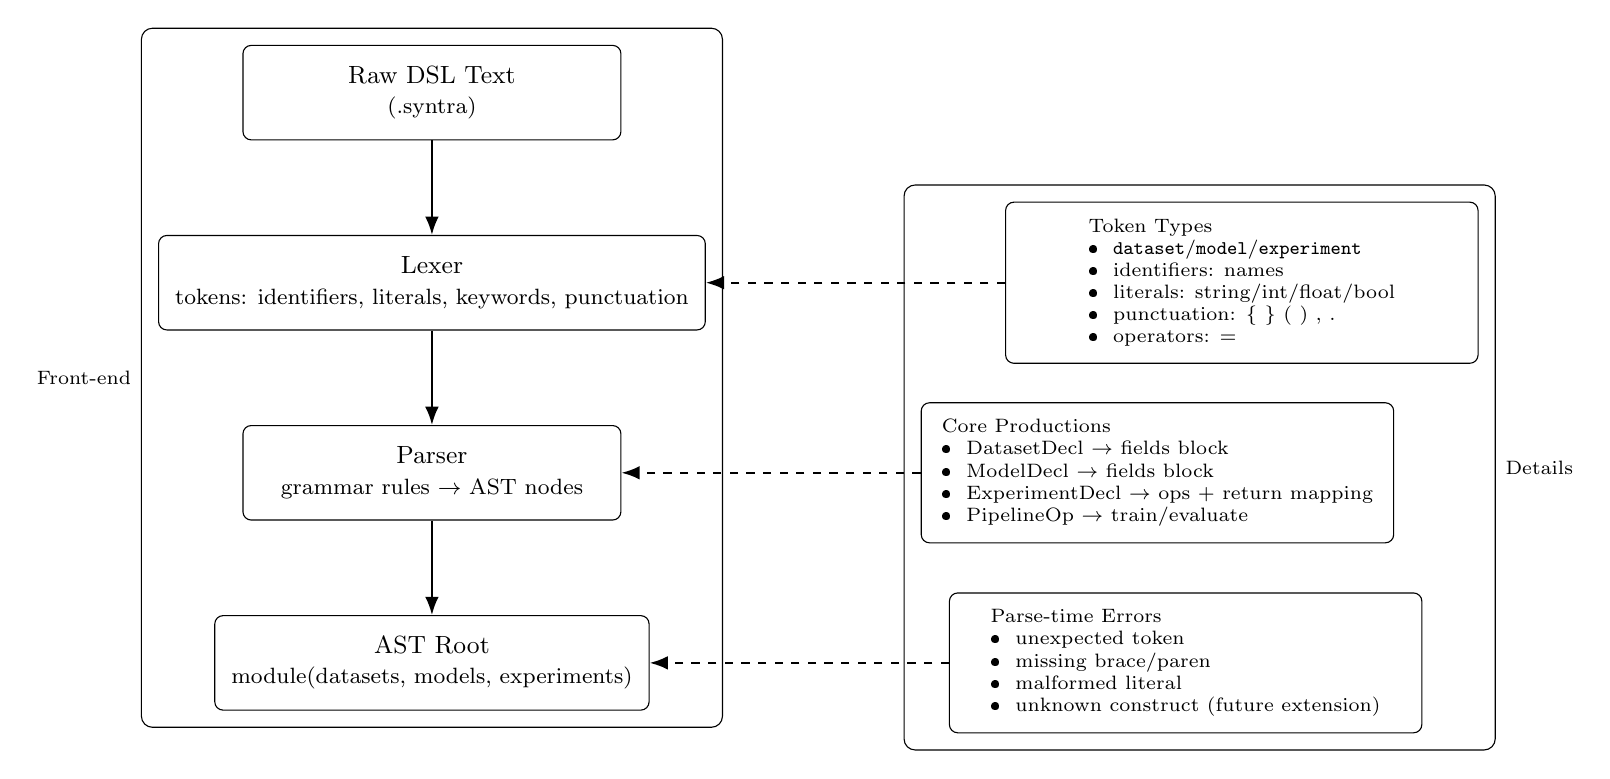
\begin{tikzpicture}[node distance=12mm]

\node[box] (raw) {Raw DSL Text\\\footnotesize (.syntra)};
\node[box, below=of raw] (lex) {Lexer\\\footnotesize tokens: identifiers, literals, keywords, punctuation};
\node[box, below=of lex] (parse) {Parser\\\footnotesize grammar rules $\rightarrow$ AST nodes};
\node[box, below=of parse] (ast) {AST Root\\\footnotesize module(datasets, models, experiments)};

% Right-side details
\node[note, right=18mm of lex, xshift=20mm] (tok) {Token Types\\
\textbullet\; \texttt{dataset}/\texttt{model}/\texttt{experiment}\\
\textbullet\; identifiers: names\\
\textbullet\; literals: string/int/float/bool\\
\textbullet\; punctuation: \{ \} ( ) , .\\
\textbullet\; operators: =};

\node[note, right=18mm of parse, xshift=20mm] (prod) {Core Productions\\
\textbullet\; DatasetDecl $\rightarrow$ fields block\\
\textbullet\; ModelDecl $\rightarrow$ fields block\\
\textbullet\; ExperimentDecl $\rightarrow$ ops + return mapping\\
\textbullet\; PipelineOp $\rightarrow$ train/evaluate};

\node[note, right=18mm of ast, xshift=20mm] (errs) {Parse-time Errors\\
\textbullet\; unexpected token\\
\textbullet\; missing brace/paren\\
\textbullet\; malformed literal\\
\textbullet\; unknown construct (future extension)};

\draw[arrow] (raw) -- (lex);
\draw[arrow] (lex) -- (parse);
\draw[arrow] (parse) -- (ast);

\draw[dashedarrow] (tok.west) -- (lex.east);
\draw[dashedarrow] (prod.west) -- (parse.east);
\draw[dashedarrow] (errs.west) -- (ast.east);

\node[group, fit=(raw)(lex)(parse)(ast), label={[font=\scriptsize]left:Front-end}] {};
\node[group, fit=(tok)(prod)(errs), label={[font=\scriptsize]right:Details}] {};

\end{tikzpicture}
\end{center}

\newpage

% =============================================================================
% Diagram 3 — AST Core Data Model (MORE DETAILED + NON-OVERLAPPING)
% =============================================================================
\section*{Diagram 3 — AST Core Data Model (Detailed Types)}

\begin{center}
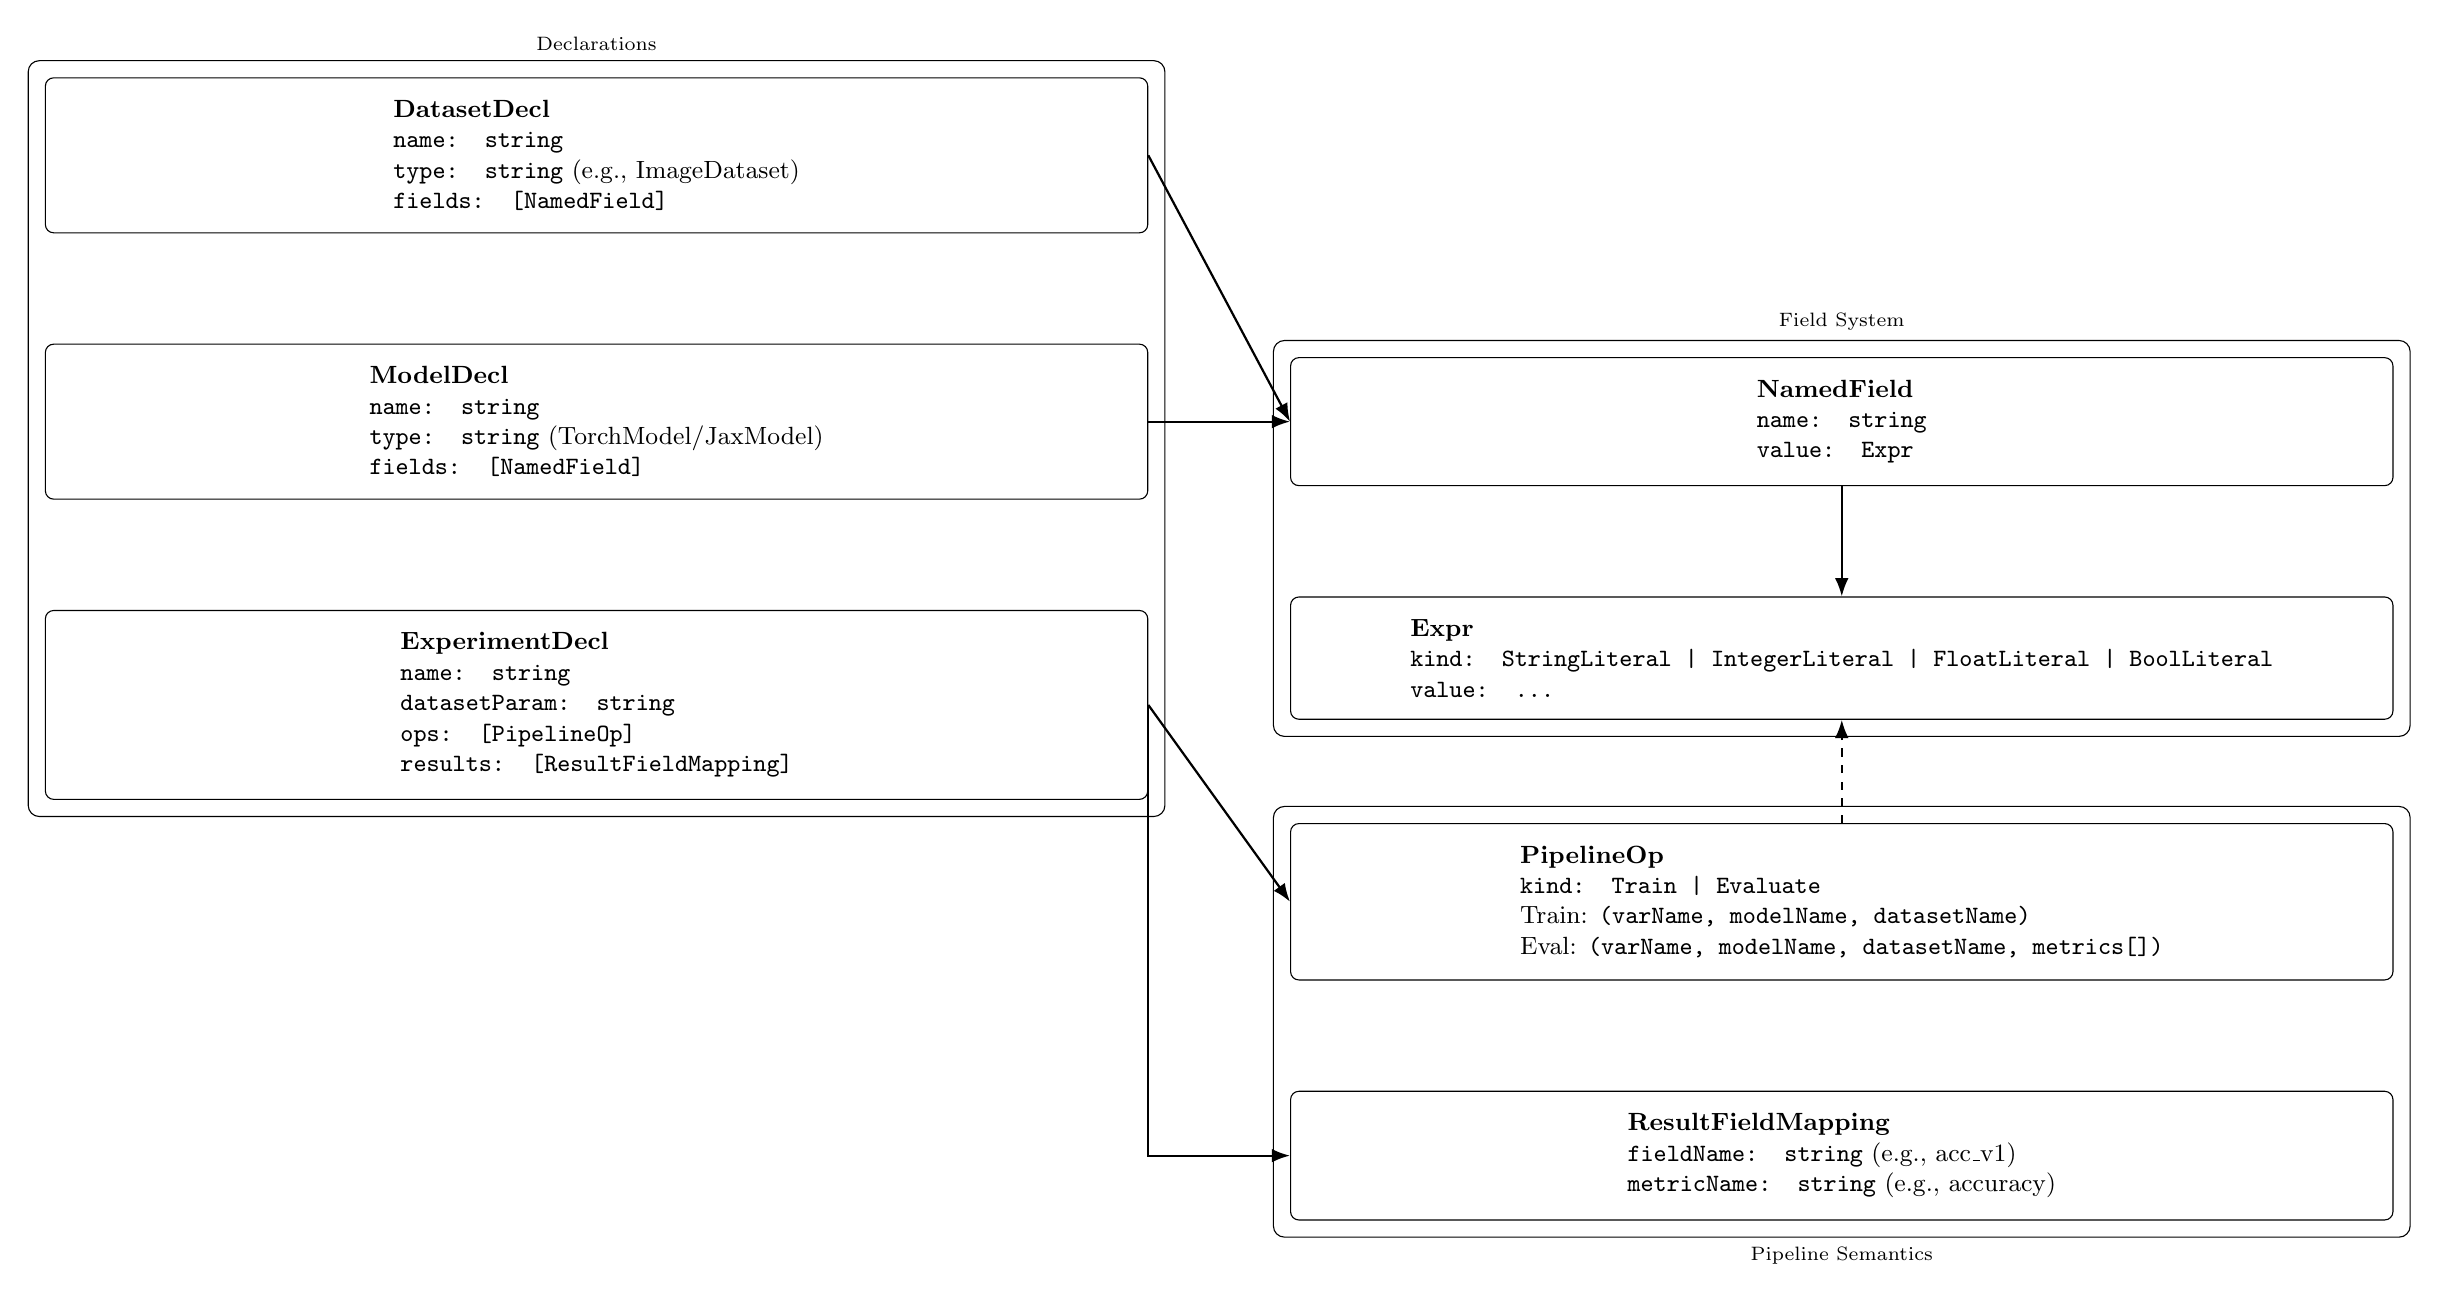
\begin{tikzpicture}[node distance=14mm]

% Left column: top-level decls
\node[wide] (ds) {\textbf{DatasetDecl}\\
\texttt{name: string}\\
\texttt{type: string} (e.g., ImageDataset)\\
\texttt{fields: [NamedField]}};

\node[wide, below=of ds] (md) {\textbf{ModelDecl}\\
\texttt{name: string}\\
\texttt{type: string} (TorchModel/JaxModel)\\
\texttt{fields: [NamedField]}};

\node[wide, below=of md] (ex) {\textbf{ExperimentDecl}\\
\texttt{name: string}\\
\texttt{datasetParam: string}\\
\texttt{ops: [PipelineOp]}\\
\texttt{results: [ResultFieldMapping]}};

% Middle column: NamedField + Expr
\node[wide, right=18mm of md] (nf) {\textbf{NamedField}\\
\texttt{name: string}\\
\texttt{value: Expr}};

\node[wide, below=of nf] (expr) {\textbf{Expr}\\
\texttt{kind: StringLiteral | IntegerLiteral | FloatLiteral | BoolLiteral}\\
\texttt{value: ...}};

% Right column: ops + results
\node[wide, right=18mm of ex, yshift=-25mm] (op) {\textbf{PipelineOp}\\
\texttt{kind: Train | Evaluate}\\
Train: \texttt{(varName, modelName, datasetName)}\\
Eval:  \texttt{(varName, modelName, datasetName, metrics[])}};

\node[wide, below=of op] (rf) {\textbf{ResultFieldMapping}\\
\texttt{fieldName: string} (e.g., acc\_v1)\\
\texttt{metricName: string} (e.g., accuracy)};

% Edges
\draw[arrow] (ds.east) -- (nf.west);
\draw[arrow] (md.east) -- (nf.west);
\draw[arrow] (nf.south) -- (expr.north);
\draw[arrow] (ex.east) -- (op.west);
\draw[arrow] (ex.east) |- (rf.west);
\draw[dashedarrow] (op.north) -- (expr.south);

% Group boxes
\node[group, fit=(ds)(md)(ex), label={[font=\scriptsize]above:Declarations}] {};
\node[group, fit=(nf)(expr), label={[font=\scriptsize]above:Field System}] {};
\node[group, fit=(op)(rf), label={[font=\scriptsize]below:Pipeline Semantics}] {};

\end{tikzpicture}
\end{center}

\newpage

% =============================================================================
% Diagram 4 — Semantic Analysis Pipeline (DETAILED)
% =============================================================================
\section*{Diagram 4 — Semantic Analysis (Validation + Normalization + Resolution)}

\begin{center}
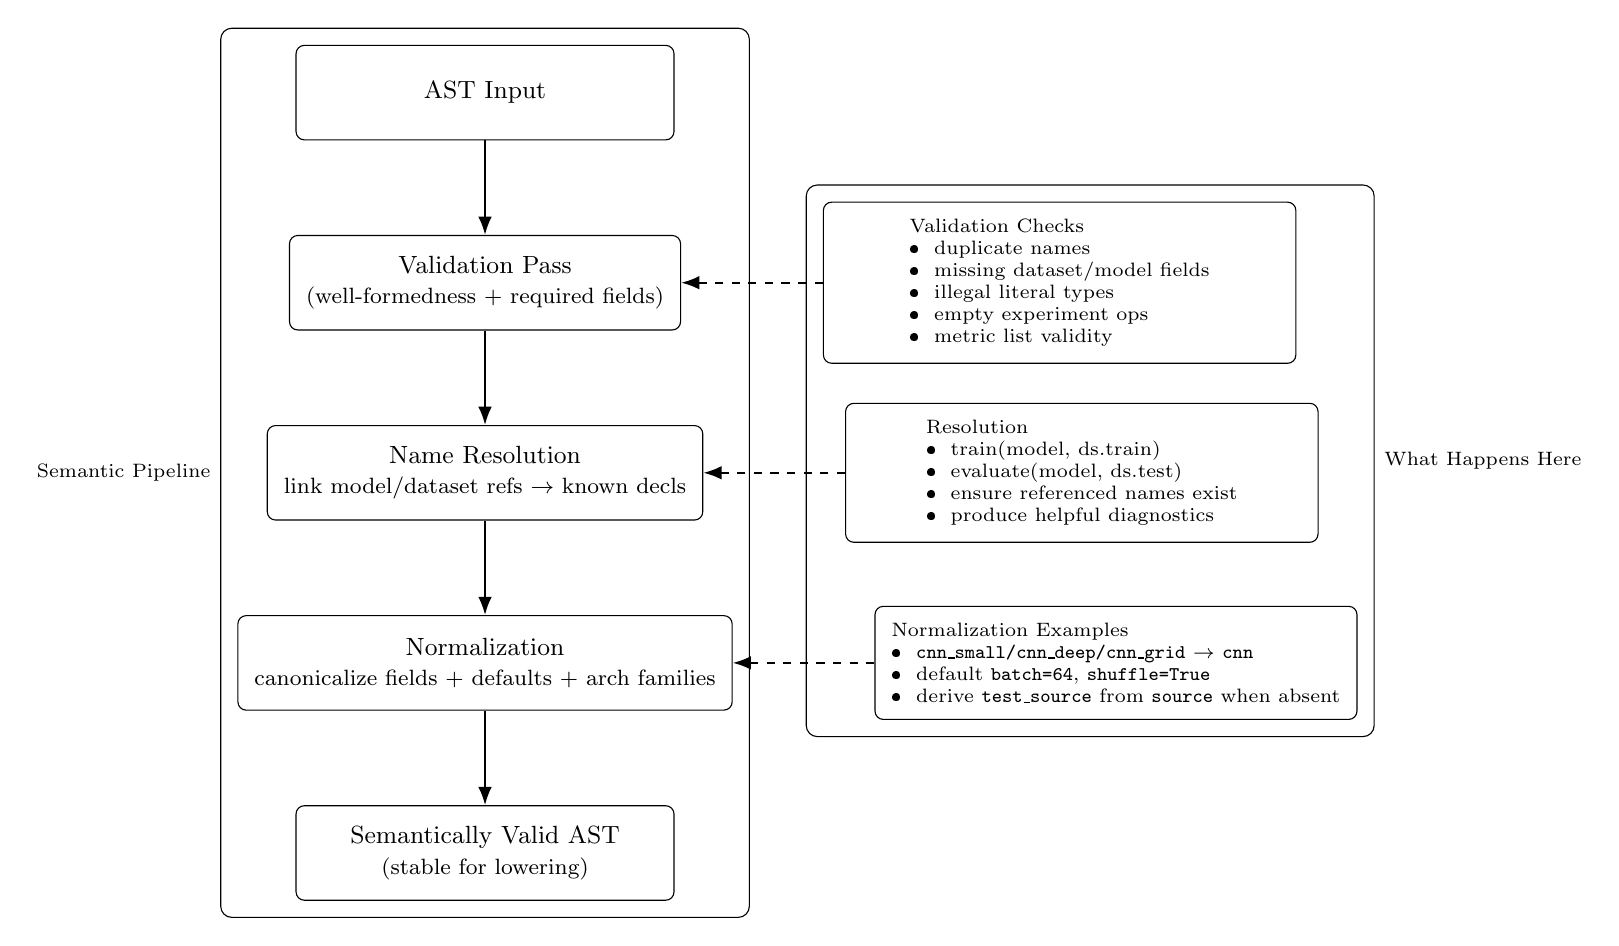
\begin{tikzpicture}[node distance=12mm]

\node[box] (astin) {AST Input};
\node[box, below=of astin] (validate) {Validation Pass\\\footnotesize (well-formedness + required fields)};
\node[box, below=of validate] (resolve) {Name Resolution\\\footnotesize link model/dataset refs $\rightarrow$ known decls};
\node[box, below=of resolve] (normalize) {Normalization\\\footnotesize canonicalize fields + defaults + arch families};
\node[box, below=of normalize] (astout) {Semantically Valid AST\\\footnotesize (stable for lowering)};

% Side notes
\node[note, right=18mm of validate] (vdet) {Validation Checks\\
\textbullet\; duplicate names\\
\textbullet\; missing dataset/model fields\\
\textbullet\; illegal literal types\\
\textbullet\; empty experiment ops\\
\textbullet\; metric list validity};

\node[note, right=18mm of resolve] (rdet) {Resolution\\
\textbullet\; train(model, ds.train)\\
\textbullet\; evaluate(model, ds.test)\\
\textbullet\; ensure referenced names exist\\
\textbullet\; produce helpful diagnostics};

\node[note, right=18mm of normalize] (ndet) {Normalization Examples\\
\textbullet\; \texttt{cnn\_small/cnn\_deep/cnn\_grid} $\rightarrow$ \texttt{cnn}\\
\textbullet\; default \texttt{batch=64}, \texttt{shuffle=True}\\
\textbullet\; derive \texttt{test\_source} from \texttt{source} when absent};

\draw[arrow] (astin) -- (validate);
\draw[arrow] (validate) -- (resolve);
\draw[arrow] (resolve) -- (normalize);
\draw[arrow] (normalize) -- (astout);

\draw[dashedarrow] (vdet.west) -- (validate.east);
\draw[dashedarrow] (rdet.west) -- (resolve.east);
\draw[dashedarrow] (ndet.west) -- (normalize.east);

\node[group, fit=(astin)(validate)(resolve)(normalize)(astout), label={[font=\scriptsize]left:Semantic Pipeline}] {};
\node[group, fit=(vdet)(rdet)(ndet), label={[font=\scriptsize]right:What Happens Here}] {};

\end{tikzpicture}
\end{center}

\newpage

% =============================================================================
% Diagram 5 — AST to IR Lowering (DETAILED)
% =============================================================================
\section*{Diagram 5 — AST to IR Lowering (Datasets/Models/Experiments)}

\begin{center}
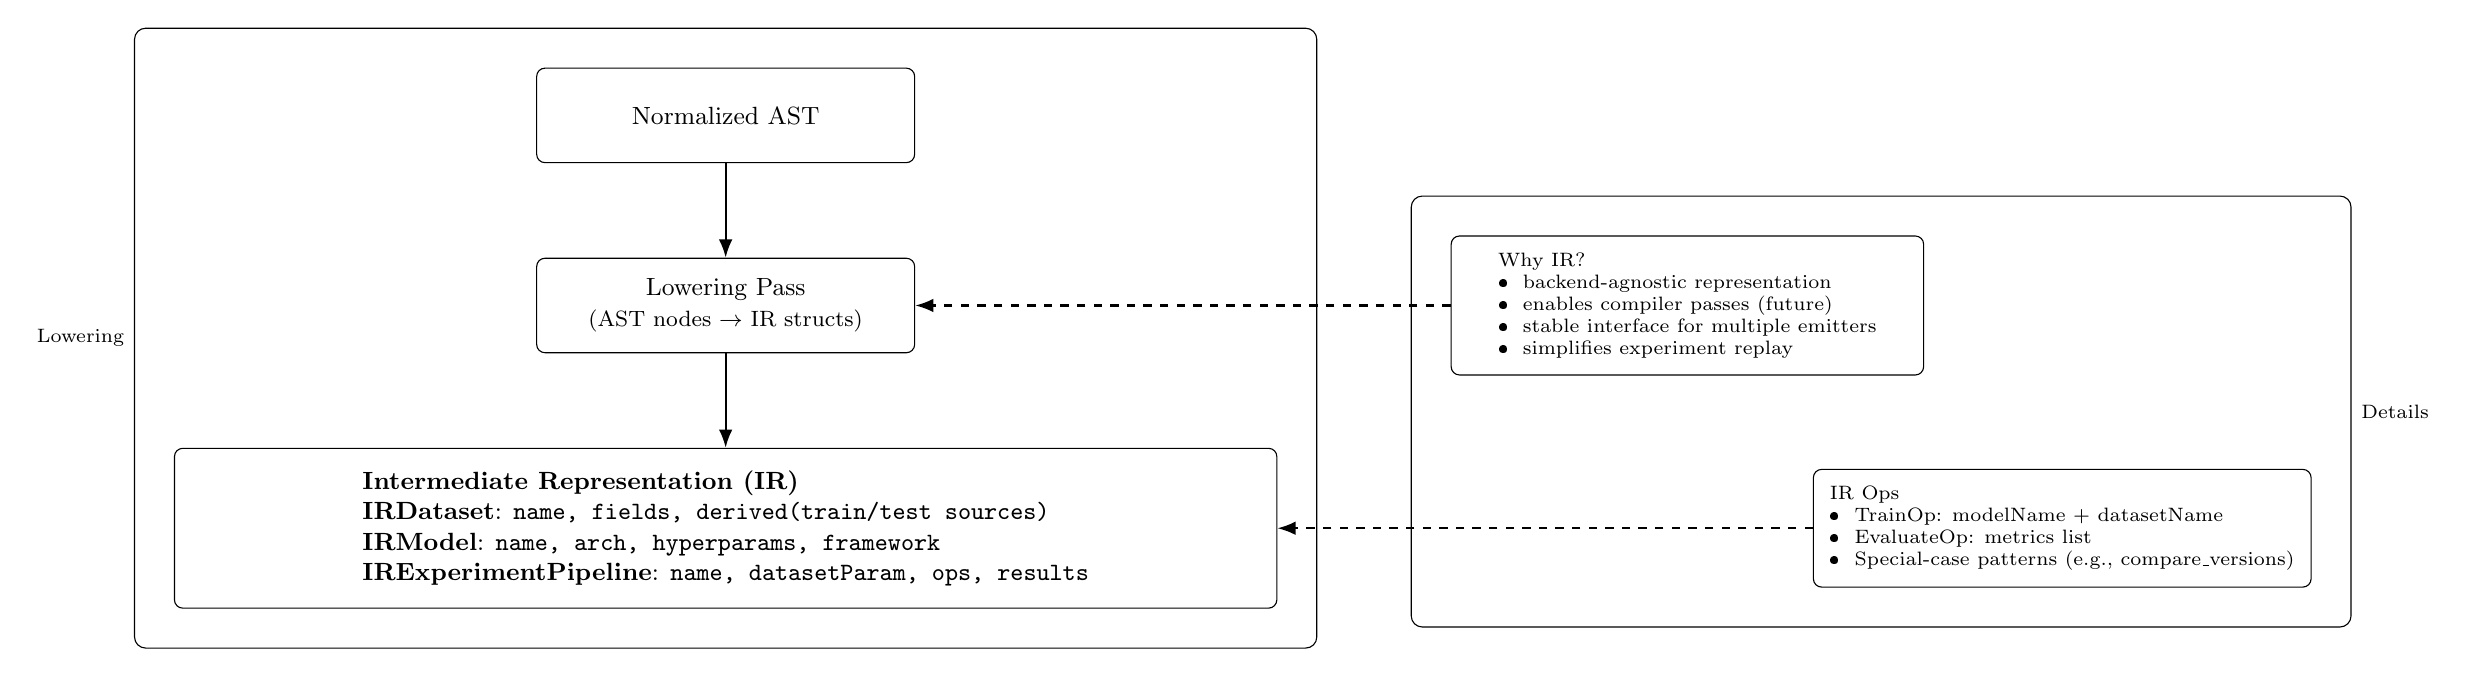
\begin{tikzpicture}[node distance=12mm]

\node[box] (ast) {Normalized AST};
\node[box, below=of ast] (lower) {Lowering Pass\\\footnotesize (AST nodes $\rightarrow$ IR structs)};
\node[wide, below=of lower] (ir) {\textbf{Intermediate Representation (IR)}\\
\textbf{IRDataset}: \texttt{name, fields, derived(train/test sources)}\\
\textbf{IRModel}: \texttt{name, arch, hyperparams, framework}\\
\textbf{IRExperimentPipeline}: \texttt{name, datasetParam, ops, results}};

% --- Push the DETAILS cluster to the right ---
\node[note, right=18mm of lower, xshift=50mm] (irdet) {Why IR?\\
\textbullet\; backend-agnostic representation\\
\textbullet\; enables compiler passes (future)\\
\textbullet\; stable interface for multiple emitters\\
\textbullet\; simplifies experiment replay};

\node[note, right=18mm of ir, xshift=50mm] (ops) {IR Ops\\
\textbullet\; TrainOp: modelName + datasetName\\
\textbullet\; EvaluateOp: metrics list\\
\textbullet\; Special-case patterns (e.g., compare\_versions)};

\draw[arrow] (ast) -- (lower);
\draw[arrow] (lower) -- (ir);

% dashed arrows still work; they just get longer
\draw[dashedarrow] (irdet.west) -- (lower.east);
\draw[dashedarrow] (ops.west) -- (ir.east);

% --- Fit groups with sane padding (slightly smaller helps avoid collision) ---
\node[group, fit=(ast)(lower)(ir), inner sep=5mm,
      label={[font=\scriptsize]left:Lowering}] {};

\node[group, fit=(irdet)(ops), inner sep=5mm,
      label={[font=\scriptsize]right:Details}] {};

\end{tikzpicture}
\end{center}

\newpage

% =============================================================================
% Diagram 6 — Backend Code Generation (DETAILED INTERNALS)
% =============================================================================
\section*{Diagram 6 — Backend Code Generation (Emitter Internals)}

\begin{center}
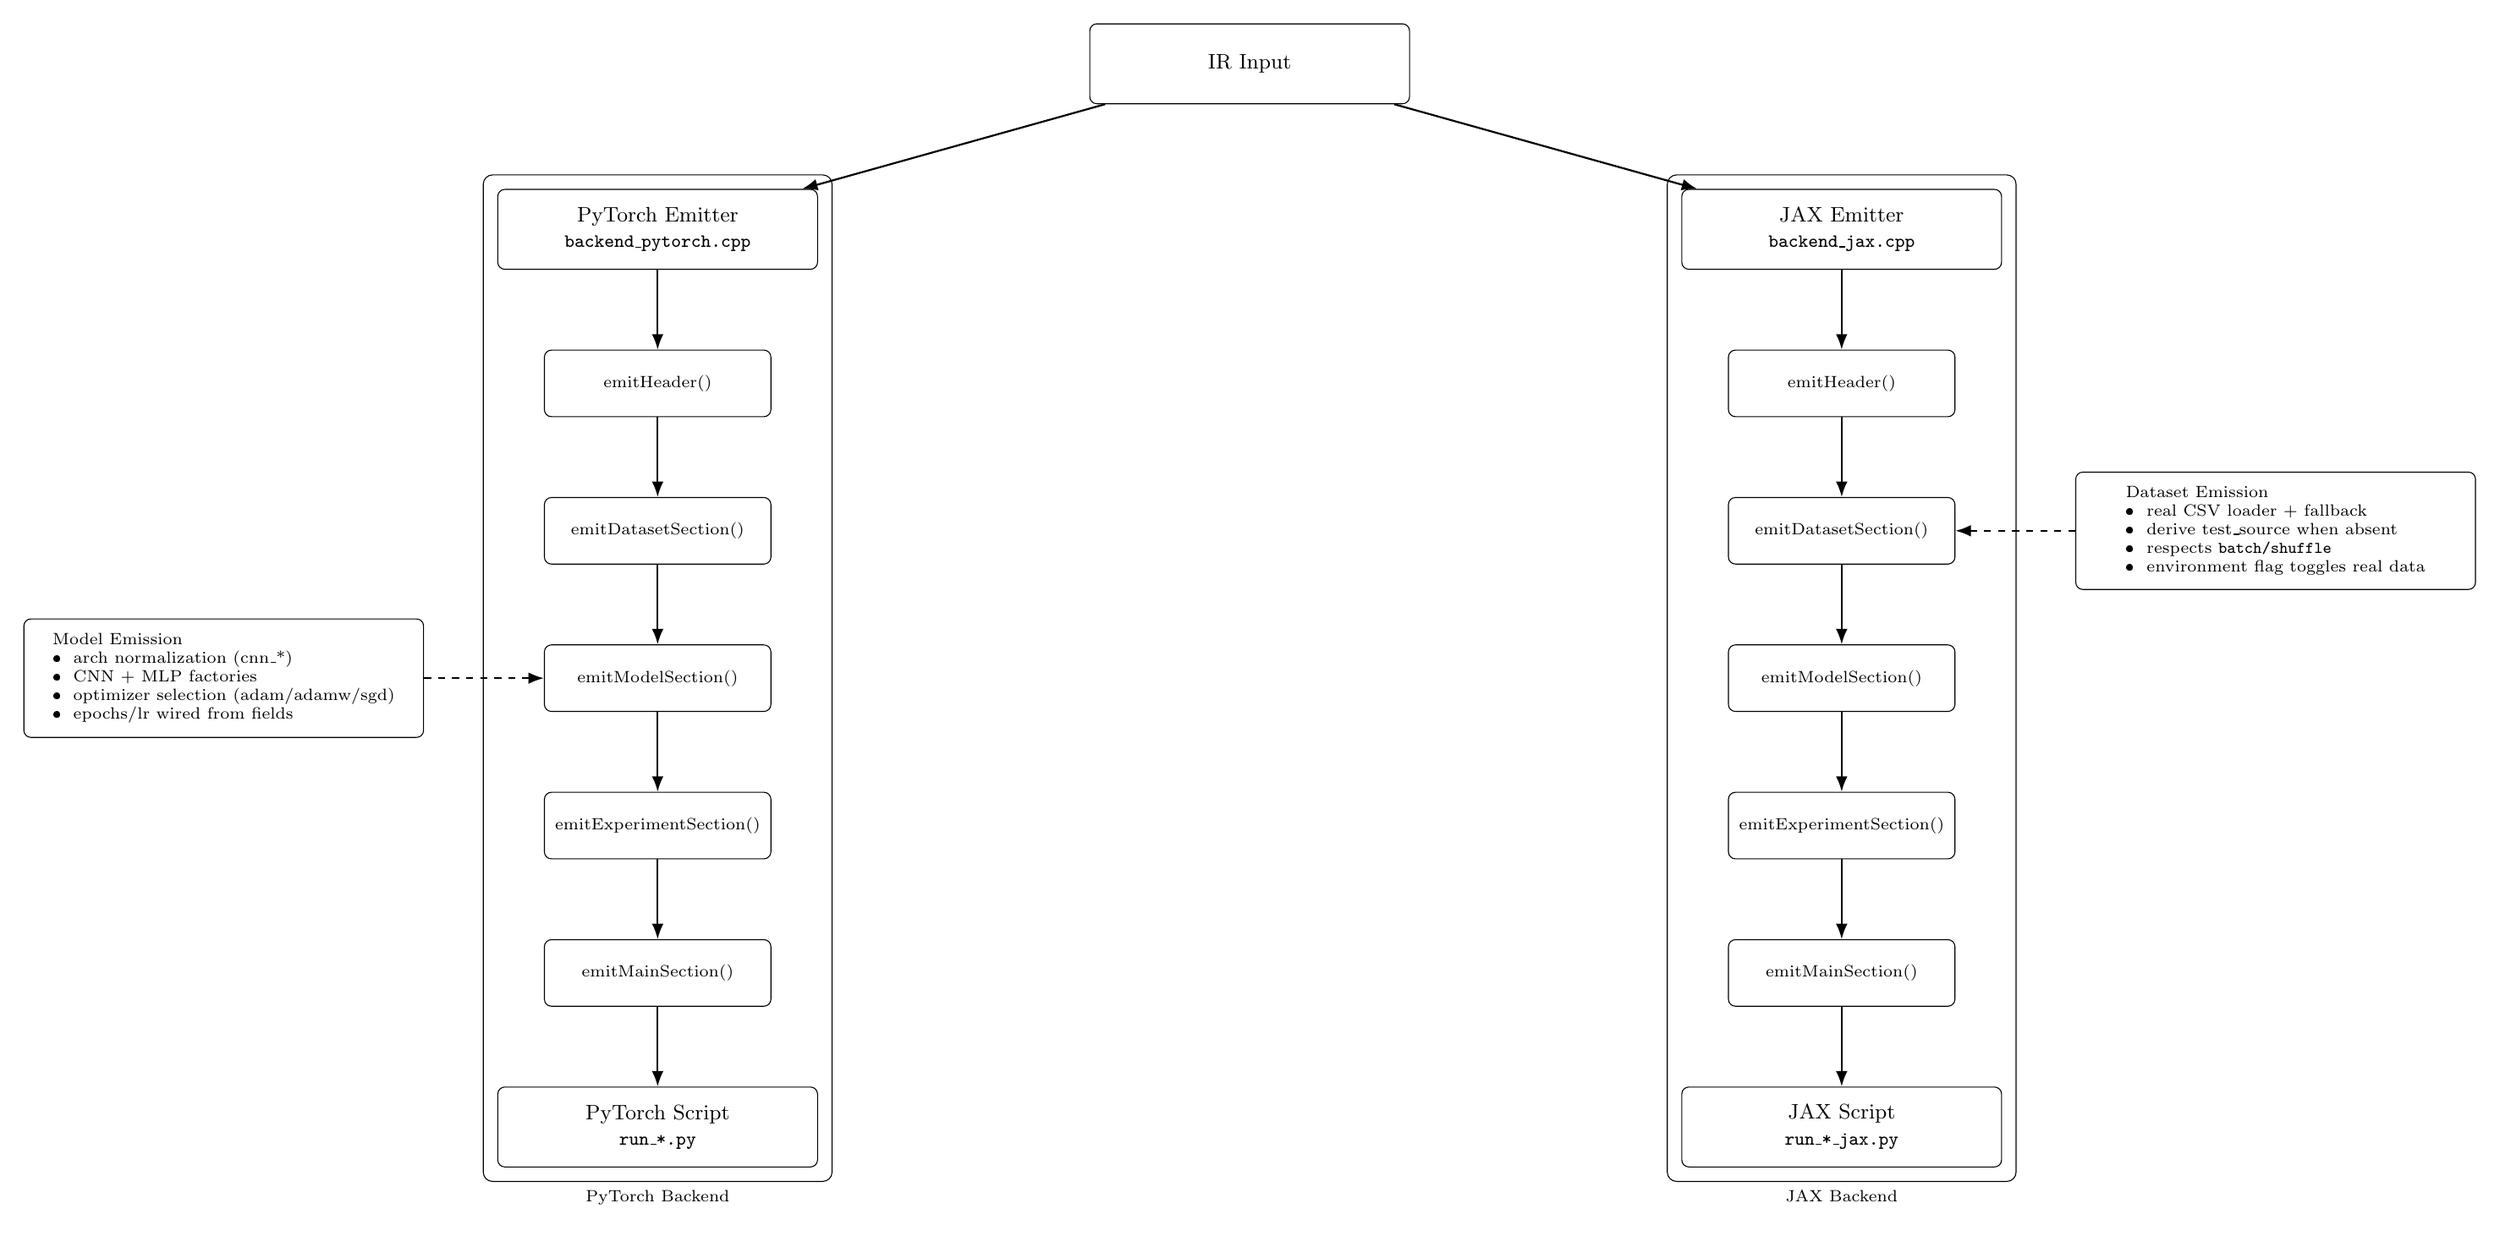
\begin{tikzpicture}[node distance=12mm]

\node[box] (ir) {IR Input};

% PyTorch emitter internals
\node[box, below left=18mm of ir, xshift=-28mm] (pt) {PyTorch Emitter\\\footnotesize \texttt{backend\_pytorch.cpp}};
\node[small, below=of pt] (pt_h) {emitHeader()};
\node[small, below=of pt_h] (pt_ds) {emitDatasetSection()};
\node[small, below=of pt_ds] (pt_m) {emitModelSection()};
\node[small, below=of pt_m] (pt_e) {emitExperimentSection()};
\node[small, below=of pt_e] (pt_main) {emitMainSection()};

\node[box, below=12mm of pt_main] (pt_out) {PyTorch Script\\\footnotesize \texttt{run\_*.py}};

% JAX emitter internals
\node[box, below right=18mm of ir, xshift=28mm] (jx) {JAX Emitter\\\footnotesize \texttt{backend\_jax.cpp}};
\node[small, below=of jx] (jx_h) {emitHeader()};
\node[small, below=of jx_h] (jx_ds) {emitDatasetSection()};
\node[small, below=of jx_ds] (jx_m) {emitModelSection()};
\node[small, below=of jx_m] (jx_e) {emitExperimentSection()};
\node[small, below=of jx_e] (jx_main) {emitMainSection()};

\node[box, below=12mm of jx_main] (jx_out) {JAX Script\\\footnotesize \texttt{run\_*\_jax.py}};

% Notes
\node[note, right=18mm of jx_ds] (dsnote) {Dataset Emission\\
\textbullet\; real CSV loader + fallback\\
\textbullet\; derive test\_source when absent\\
\textbullet\; respects \texttt{batch/shuffle}\\
\textbullet\; environment flag toggles real data};

\node[note, left=18mm of pt_m] (mnote) {Model Emission\\
\textbullet\; arch normalization (cnn\_*)\\
\textbullet\; CNN + MLP factories\\
\textbullet\; optimizer selection (adam/adamw/sgd)\\
\textbullet\; epochs/lr wired from fields};

% Connections
\draw[arrow] (ir) -- (pt);
\draw[arrow] (ir) -- (jx);

\draw[arrow] (pt) -- (pt_h);
\draw[arrow] (pt_h) -- (pt_ds);
\draw[arrow] (pt_ds) -- (pt_m);
\draw[arrow] (pt_m) -- (pt_e);
\draw[arrow] (pt_e) -- (pt_main);
\draw[arrow] (pt_main) -- (pt_out);

\draw[arrow] (jx) -- (jx_h);
\draw[arrow] (jx_h) -- (jx_ds);
\draw[arrow] (jx_ds) -- (jx_m);
\draw[arrow] (jx_m) -- (jx_e);
\draw[arrow] (jx_e) -- (jx_main);
\draw[arrow] (jx_main) -- (jx_out);

\draw[dashedarrow] (mnote.east) -- (pt_m.west);
\draw[dashedarrow] (dsnote.west) -- (jx_ds.east);

\node[group, fit=(pt)(pt_h)(pt_ds)(pt_m)(pt_e)(pt_main)(pt_out), label={[font=\scriptsize]below:PyTorch Backend}] {};
\node[group, fit=(jx)(jx_h)(jx_ds)(jx_m)(jx_e)(jx_main)(jx_out), label={[font=\scriptsize]below:JAX Backend}] {};

\end{tikzpicture}
\end{center}

\newpage

% =============================================================================
% Diagram 7 — Runtime Execution (DETAILED + REAL/FALLBACK DATA PATHS)
% =============================================================================
\section*{Diagram 7 — Generated Script Runtime Execution (Real Data vs Fallback)}

\begin{center}
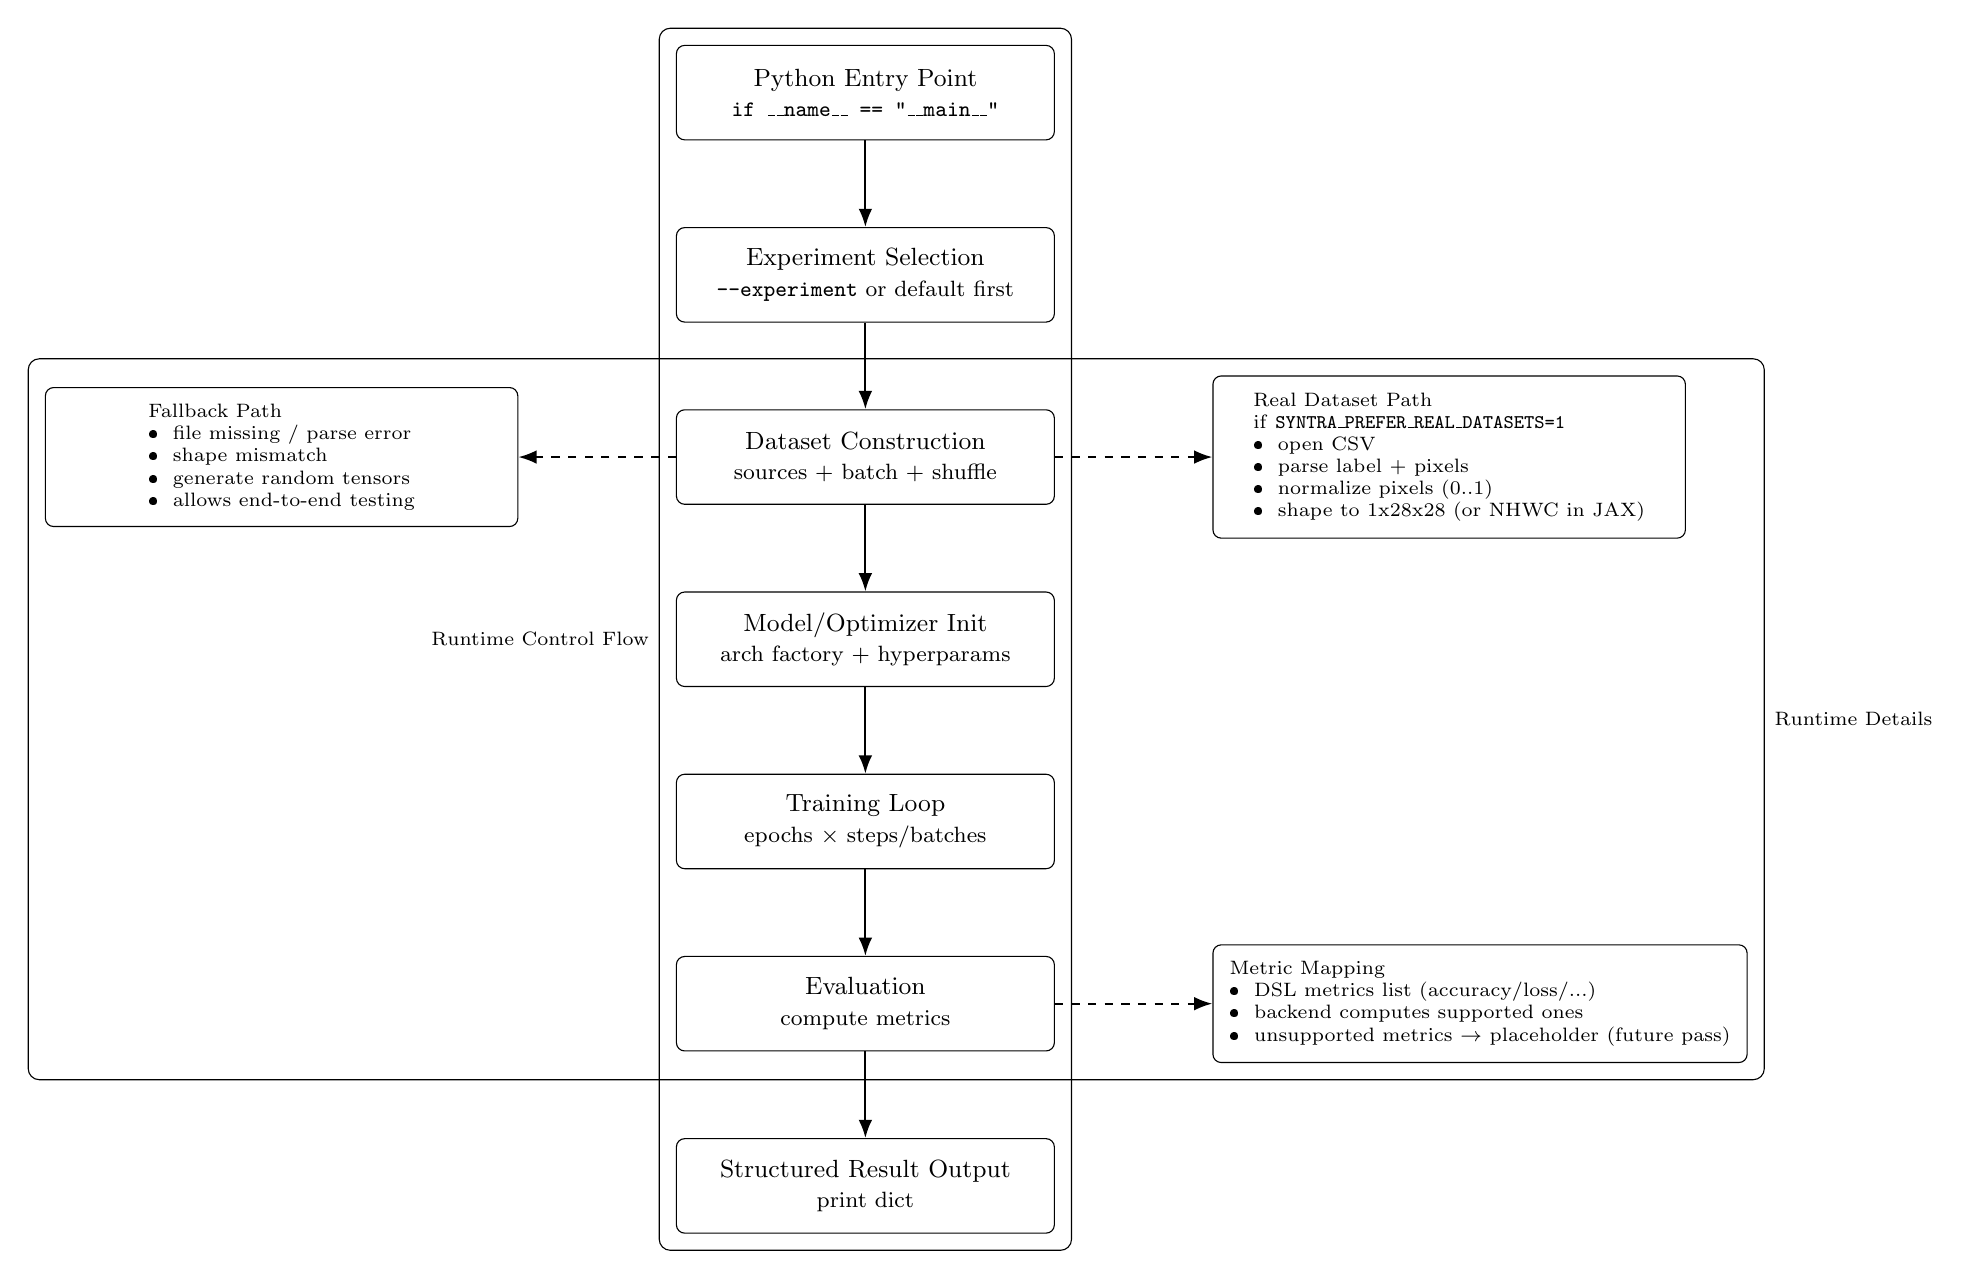
\begin{tikzpicture}[node distance=11mm]

\node[box] (start) {Python Entry Point\\\footnotesize \texttt{if \_\_name\_\_ == "\_\_main\_\_"}};
\node[box, below=of start] (pick) {Experiment Selection\\\footnotesize \texttt{--experiment} or default first};
\node[box, below=of pick] (ds) {Dataset Construction\\\footnotesize sources + batch + shuffle};
\node[box, below=of ds] (model) {Model/Optimizer Init\\\footnotesize arch factory + hyperparams};
\node[box, below=of model] (train) {Training Loop\\\footnotesize epochs $\times$ steps/batches};
\node[box, below=of train] (eval) {Evaluation\\\footnotesize compute metrics};
\node[box, below=of eval] (out) {Structured Result Output\\\footnotesize print dict};

% Branch details for dataset loading
\node[note, right=20mm of ds] (real) {Real Dataset Path\\
if \texttt{SYNTRA\_PREFER\_REAL\_DATASETS=1}\\
\textbullet\; open CSV\\
\textbullet\; parse label + pixels\\
\textbullet\; normalize pixels (0..1)\\
\textbullet\; shape to 1x28x28 (or NHWC in JAX)};

\node[note, left=20mm of ds] (stub) {Fallback Path\\
\textbullet\; file missing / parse error\\
\textbullet\; shape mismatch\\
\textbullet\; generate random tensors\\
\textbullet\; allows end-to-end testing};

% Metrics mapping note
\node[note, right=20mm of eval] (metrics) {Metric Mapping\\
\textbullet\; DSL metrics list (accuracy/loss/...)\\
\textbullet\; backend computes supported ones\\
\textbullet\; unsupported metrics $\rightarrow$ placeholder (future pass)};

% Arrows main flow
\draw[arrow] (start) -- (pick);
\draw[arrow] (pick) -- (ds);
\draw[arrow] (ds) -- (model);
\draw[arrow] (model) -- (train);
\draw[arrow] (train) -- (eval);
\draw[arrow] (eval) -- (out);

% Branch arrows
\draw[dashedarrow] (ds.east) -- (real.west);
\draw[dashedarrow] (ds.west) -- (stub.east);
\draw[dashedarrow] (eval.east) -- (metrics.west);

\node[group, fit=(start)(pick)(ds)(model)(train)(eval)(out), label={[font=\scriptsize]left:Runtime Control Flow}] {};
\node[group, fit=(real)(stub)(metrics), label={[font=\scriptsize]right:Runtime Details}] {};

\end{tikzpicture}
\end{center}

\end{document}